\documentclass{article}
\usepackage{graphicx}
\graphicspath{ {images/} }
\usepackage[utf8]{inputenc}

\title{CIS 510 Final Project}
\author{Areej Alghamdi and Jacob Lambert}
\date{\today}


\begin{document}
\maketitle

Although we each implemented only certain features separately, we met several times to discuss the design and implementation of all the features. Jacob primarily worked on creating the face mesh, designing the Qt GUI, and setting up the callbacks in python. Areej primarily worked on creating individual deformers for each metric, and ensuring that the deformers worked together as required.

\section*{Maya Face Mesh} (Jacob)
To create the face mesh, I first found a crude drawing of a human head to use as an image plane in Maya. The image plane helped with modeling realistic facial dimensions. 

To begin the modeling process, I first created a polygon from the side perspective using the image plane. This polygon served as an outline of the head. After deleting extraneous faces,
I extruded this outline to begin modeling. 

For the eye and mouth areas, I created a cylinder and deleted unneeded surfaces. I then combined this cylinder with the outline mesh.

Throughout the modeling process, I attempted to use only quad faces. This required adding edge-loops and creating new polygons. Most of the polygons were created by extruding edges and merging vertices. I also used the \texttt{append-to-polygon} tool.

The eyes are spheres scaled to roughly match the size of the eye holes in the face mesh.\newline

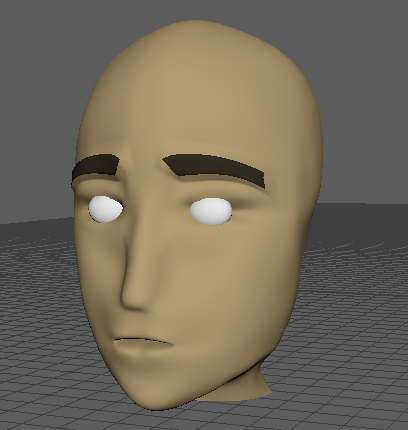
\includegraphics[scale=.4]
  {face.png}

  \subsection*{Self-critique}
  While the face does look somewhat human, it needs some improvement. Currently the model has no ears. Also, when smoothing the mesh, I did not distinguish between "soft" and "hard" edges, resulting in over-smoothing in some areas.
  
\section*{Maya Individual Deformations} (Areej)

  \subsection*{Self-critique}

\section*{Maya Linking Deformations} (Areej)

  \subsection*{Self-critique}

\section*{Qt GUI} (Jacob)
The Qt GUI consists is relatively simple. It consists of a text label and slider for each modifiable attribute. The label contains the name of the attribute and the current value assigned to the attribute. The slider ranges from -1 to 1, and is initialized to zero. The magnitude of the value of the slider represents the value of the associated attribute. The GUI also contains buttons to generate a random
face and capture a screenshot.\newline

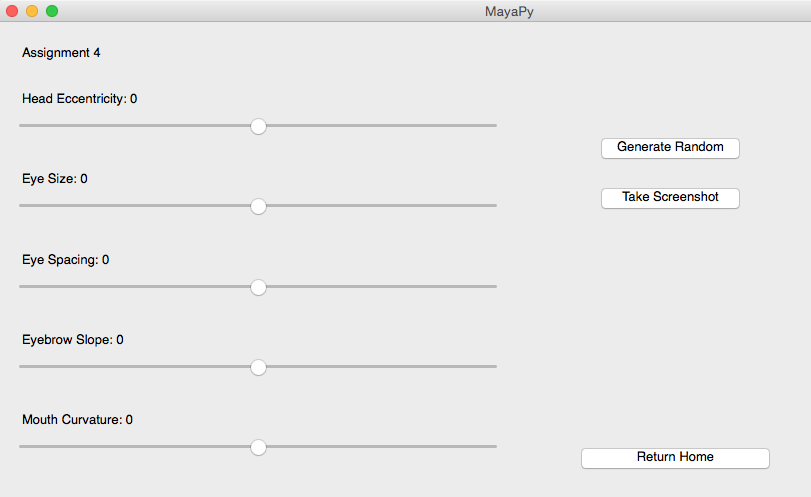
\includegraphics[scale=.4]
  {gui.png}
  \subsection*{Self-critique}
  The GUI could allow users to manually input values for the attributes in addition to using the slider. This would require a more MVC based design to keep the slider and user-input values consistent.

\section*{Python} (Jacob)
Each element of the GUI
has a corresponding event 
handler within in python. For the sliders, the handler gets the value from the slider, and applies the appropriate blend shape proportionally to the value. Some sliders have two
associated blendshapes. For example, the \texttt{Mouth Curvature} slider applies the \texttt{Smile} blendshape for positive values and the \texttt{Frown} blendshape for negative values.

The sliders that affect the eyes also translate and scale the eye polygons, in addition to applying the appropriate blendshapes to the face mesh.

The \texttt{Generate Random} button generates random values for all of the sliders using python's random number generator. The 
\texttt{Take Screenshot} button allows you to select a region of the screen to save as \texttt{{\raise.17ex\hbox{$\scriptstyle\sim$}}/Desktop/faceN.png}, where \texttt{N} is the number of screenshots taken.

  \subsection*{Self-critique} The translation of the eyes is currently dependant on the absolute position of the polygons in the world. It would be nice to somehow make this translation keyed or relative to the location of the face mesh. Additionaly the eye polygons do not match the mesh exactly for all
  face configurations.
  
  Also, \texttt{Take Screenshot} is probably not portable, as it relies on the OSX specific \texttt{screencast} program.

\end{document}
